\documentclass[tikz,border=5pt]{standalone}
\usepackage{xcolor}
\usepackage{tikz}

\begin{document}
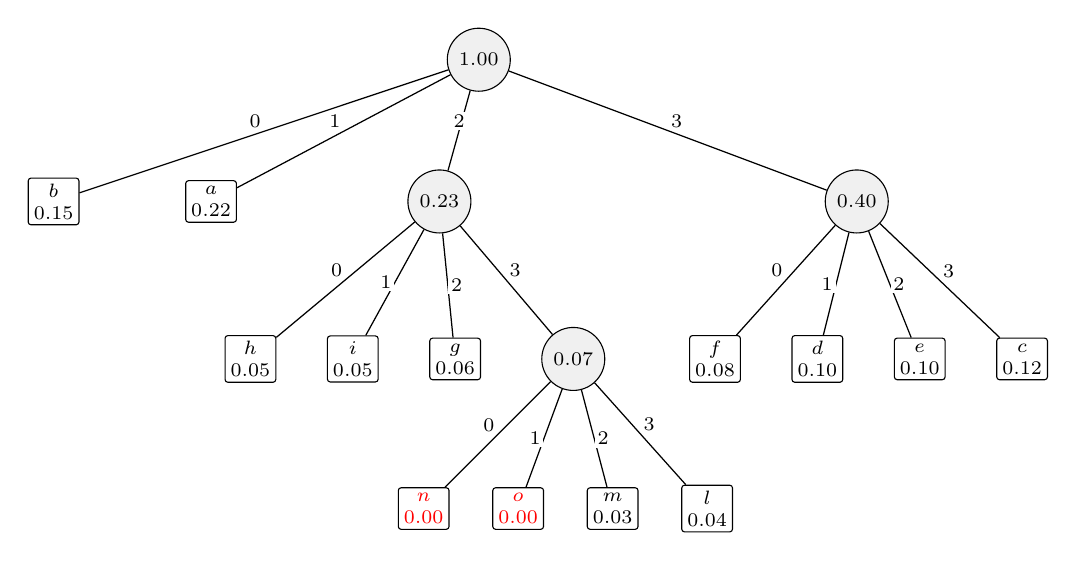
\begin{tikzpicture}[
    % Stili comuni per nodi, archi ed etichette dell'albero.
    edge/.style={draw, line width=0.45pt},
    every node/.style={font=\scriptsize, align=center},
    edge label/.style={font=\scriptsize, inner sep=1pt, fill=white},
    internal/.style={circle, draw, fill=black!6, minimum size=8mm, inner sep=1pt},
    leaf/.style={rectangle, draw, rounded corners=1pt, fill=white, inner sep=2pt},
    dummy leaf/.style={leaf, text=red}
]
% Albero di Huffman quaternario per la sorgente:
% a,b,c,d,e,f,g,h,i,l,m,n,o con n,o simboli fittizi di probabilita' 0.

% Nodi principali, posizionati manualmente per mantenere leggibile il ramo 4-ario.
\node[internal] (root) at (0, 0) {$1.00$};

\node[leaf]     (b) at (-5.4, -1.8) {$b$\\$0.15$};
\node[leaf]     (a) at (-3.4, -1.8) {$a$\\$0.22$};
\node[internal] (B) at (-0.5, -1.8) {$0.23$};
\node[internal] (C) at (4.8, -1.8) {$0.40$};

\node[leaf]     (h) at (-2.9, -3.8) {$h$\\$0.05$};
\node[leaf]     (i) at (-1.6, -3.8) {$i$\\$0.05$};
\node[leaf]     (g) at (-0.3, -3.8) {$g$\\$0.06$};
\node[internal] (A) at (1.2, -3.8) {$0.07$};

\node[leaf]     (f) at (3.0, -3.8) {$f$\\$0.08$};
\node[leaf]     (d) at (4.3, -3.8) {$d$\\$0.10$};
\node[leaf]     (e) at (5.6, -3.8) {$e$\\$0.10$};
\node[leaf]     (c) at (6.9, -3.8) {$c$\\$0.12$};

\node[dummy leaf] (n) at (-0.7, -5.7) {$n$\\$0.00$};
\node[dummy leaf] (o) at (0.5, -5.7) {$o$\\$0.00$};
\node[leaf]       (m) at (1.7, -5.7) {$m$\\$0.03$};
\node[leaf]       (l) at (2.9, -5.7) {$l$\\$0.04$};

% Etichette 0,1,2,3 assegnate da sinistra a destra a ogni fusione.
\draw[edge] (root) -- node[edge label, above left] {$0$} (b);
\draw[edge] (root) -- node[edge label, above left] {$1$} (a);
\draw[edge] (root) -- node[edge label, above] {$2$} (B);
\draw[edge] (root) -- node[edge label, above right] {$3$} (C);

\draw[edge] (B) -- node[edge label, above left] {$0$} (h);
\draw[edge] (B) -- node[edge label, left] {$1$} (i);
\draw[edge] (B) -- node[edge label, right] {$2$} (g);
\draw[edge] (B) -- node[edge label, above right] {$3$} (A);

\draw[edge] (C) -- node[edge label, above left] {$0$} (f);
\draw[edge] (C) -- node[edge label, left] {$1$} (d);
\draw[edge] (C) -- node[edge label, right] {$2$} (e);
\draw[edge] (C) -- node[edge label, above right] {$3$} (c);

\draw[edge] (A) -- node[edge label, above left] {$0$} (n);
\draw[edge] (A) -- node[edge label, left] {$1$} (o);
\draw[edge] (A) -- node[edge label, right] {$2$} (m);
\draw[edge] (A) -- node[edge label, above right] {$3$} (l);
\end{tikzpicture}
\end{document}
